\documentclass{article}
\usepackage{geometry}
\usepackage{tabularx}
\usepackage{array}
\usepackage{multirow}
\usepackage{makecell}
\usepackage{titlesec}
\usepackage{setspace}
\usepackage{titletoc}
\usepackage{caption}
\usepackage{graphicx}
\usepackage{enumitem}
\usepackage{bm}


\geometry{a4paper, margin=1in}
\renewcommand{\arraystretch}{1.5}

% Personalização do cabeçalho
\titleformat{\section}[block]{\normalfont\Large\bfseries\filcenter}{\thesection}{1em}{}
\titlespacing*{\section}{0pt}{*2}{*2}

\renewcommand{\contentsname}{\hfill\bfseries\Large Sumário\hfill}

% Configuração para centralizar as entradas do sumário
\titlecontents{chapter}[1em]{\vspace{1ex}}{\bfseries\Large\contentslabel{2em}\hfill}{\bfseries\Large\hfill}{\bfseries\Large\hfill\contentspage}

\captionsetup[table]{name=Tabela}





\begin{document}

\title{INSTITUTO FEDERAL DE EDUCAÇÃO, CIÊNCIA E TECNOLOGIA GOIANO (IF)\\ CAMPUS CERES\\ BACHARELADO EM SISTEMAS DE INFORMAÇÃO\\ANÁLISE DE SISTEMAS ORIENTADOS A OBJETOS}
\doublespacing
\date{}
\maketitle
\vspace{50pt}

\section*{Site: Slab}
\vspace{70pt}

\begin{center}
 \large
 \section*{Autores} 
 CARLOS HENRIQUE MOTA MARTINS\\
 ORLANDO SOARES DE SANTANA FILHO \\
 THIAGO HENRIQUE FÉLIX CÂNDIDO RIBEIRO CONCEIÇÃO\\
 MATHEUS OLIVEIRA BRANDÃO\\
 
 
\section*{CERES\\2023}
\vspace{70pt}

\tableofcontents
\end{center}
\vspace{290pt}

\section{Introdução}
{Esse documento trata da documentação da funcionalidade de login, cadastro, quiz e ranking do quiz dentro do Statistical Lab (SLab), fornecendo informações essenciais para compreensão e implementação dessas funcionalidades.}
\vspace{40pt}



\subsection{Requisitos}
\vspace{30pt}

\subsubsection{Requisitos não Funcionais}
\vspace{20pt}

\begin{center}
\large
\doublespacing
\captionof{table}{Requisito Não Funcional (RNF1) - O sistema deve ser desenvolvido em linguagem PHP na parte de comunicação do servidor com banco de dados}
\begin{tabular}{|c|p{10cm}|}
    \hline
    \textbf{Identificação do requisito} & RNF1 \\
    \hline
    \textbf{Nome do Requisito} & O sistema deve ser desenvolvido em linguagem PHP na parte de comunicação do servidor com banco de dados \\
    \hline
    \textbf{Local} & IF Goiano Ceres \\
    \hline
    \textbf{Data} & 01 de outubro de 2023 \\
    \hline
    \textbf{Responsável pelo Requisito} & Ronneesley \\
    \hline
    \multicolumn{2}{|c|}{\textbf{Especificação do Requisito}} \\
    \hline
    \multicolumn{2}{|c|}{\begin{tabular}{@{}p{10cm}@{}}Devido à capacidade de lidar com as operações de banco de dados e sua popularidade no desenvolvimento web, o PHP foi a escolha para desenvolver o Slab. \end{tabular}} \\
    \hline
\end{tabular}
\end{center}
\vspace{180pt}

\begin{center}
\large
\onehalfspacing
\captionof{table}{Requisito não Funcional (RNF2) - O sistema de gerenciamento de banco de dados (SGBD)deve ser o MySQL }
\begin{tabular}{|c|p{10cm}|}
	\hline
	\textbf{Identificação} & RNF2 \\
	\hline
	\textbf{Nome do Requisito} & O sistema de gerenciamento de banco de dados (SGBD)deve ser o MySQL \\
	\hline
	\textbf{Local} & IF Goiano Ceres \\
	\hline
	\textbf{Data} & 01 de outubro de 2023 \\
	\hline
	\textbf{Responsável pelo Requisito} & Ronneesley\\
	\hline
	\multicolumn{2}{|c|}{\textbf{Especificação do Requisito}} \\
	\hline
	\multicolumn{2}{|c|}{\begin{tabular}{@{}p{10cm}@{}}Devido a confiabilidade e compatibilidade, o MySQL foi a escolha mais viável para esse sistema web. \end{tabular}} \\
	\hline
\end{tabular}
\end{center}
\vspace{20pt}

\begin{center}
\large
\onehalfspacing
\captionof{table}{Requisito não Funcional (RNF3) - O sistema deve funcionar na web}
\begin{tabular}{|c|p{10cm}|}
	\hline
	\textbf{Identificação} & RNF3 \\
	\hline
	\textbf{Nome do Requisito} & O sistema deve funcionar na web \\
	\hline
	\textbf{Local} & IF Goiano Ceres \\
	\hline
	\textbf{Data} & 01 de outubro de 2023 \\
	\hline
	\textbf{Responsável pelo Requisito} & Ronneesley\\
	\hline
	\multicolumn{2}{|c|}{\textbf{Especificação do Requisito}} \\
	\hline
	\multicolumn{2}{|c|}{\begin{tabular}{@{}p{10cm}@{}}Sistema deve ser acessível via navegador web para garantir um fácil acesso.  \end{tabular}} \\
	\hline
\end{tabular}
\end{center}
\vspace{130pt}

\begin{center}
\large
\onehalfspacing
\captionof{table}{Requisito não Funcional (RNF4) - O sistema deve ser desenvolvido na camada de interface do usuário utilizando tecnologias web padrão, como HTML, CSS e JavaScript}
\begin{tabular}{|c|p{10cm}|}
	\hline
	\textbf{Identificação} & RNF4 \\
	\hline
	\textbf{Nome do Requisito} & O sistema deve ser desenvolvido na camada de interface do usuário utilizando tecnologias web padrão, como HTML, CSS e JavaScript\\
	\hline
	\textbf{Local} & IF Goiano Ceres \\
	\hline
	\textbf{Data} & 01 de outubro de 2023 \\
	\hline
	\textbf{Responsável pelo Requisito} & Ronneesley \\
	\hline
	\multicolumn{2}{|c|}{\textbf{Especificação do Requisito}} \\
	\hline
	\multicolumn{2}{|c|}{\begin{tabular}{@{}p{10cm}@{}}A escolha das tecnologias HTML, CSS e JavaScript para o front-end fundamenta-se na capacidade do HTML para estruturar de forma semântica, no poder do CSS para estilização flexível e adaptável, e na versatilidade do JavaScript para adicionar dinamismo e interatividade, garantindo uma experiência de usuário moderna, acessível e eficiente. \end{tabular}} \\
	\hline
\end{tabular}
\end{center}


\subsubsection{Requisitos funcionais}
\begin{center}
\large
\onehalfspacing
\captionof{table}{Requisito Funcional (RF1) - O sistema deve fornecer um cadastro completo e funcional}
\begin{tabular}{|c|p{10cm}|}
	\hline
	\textbf{Identificação} & RF1 \\
	\hline
	\textbf{Nome do Requisito} &  O sistema deve fornecer um cadastro completo e funcional \\
	\hline
	\textbf{Local} & IF Goiano Ceres \\
	\hline
	\textbf{Data} & 01 de outubro de 2023 \\
	\hline
	\textbf{Responsável pelo Requisito} & Orlando e Thiago\\
	\hline
	\multicolumn{2}{|c|}{\textbf{Especificação do Requisito}} \\
	\hline
	\multicolumn{2}{|c|}{\begin{tabular}{@{}p{10cm}@{}}Para que os internautas consigam entrar no sistema com o login e necessário a interface para que os dados necessários sejam inseridos no banco de dados. \end{tabular}} \\
	\hline
\end{tabular}
\end{center}




\begin{center}
\large
\onehalfspacing
\captionof{table}{Requisito Funcional (RF2) - O sistema deve fornecer uma listagem de cursos no cadastro}
\begin{tabular}{|c|p{10cm}|}
	\hline
	\textbf{Identificação} & RF2 \\
	\hline
	\textbf{Nome do Requisito} & O sistema deve fornecer uma listagem de cursos no cadastro\\
	\hline
	\textbf{Local} & IF Goiano Ceres \\
	\hline
	\textbf{Data} & 01 de outubro de 2023 \\
	\hline
	\textbf{Responsável pelo Requisito}&  Orlando e Thiago \\
	\hline
	\multicolumn{2}{|c|}{\textbf{Especificação do Requisito}} \\
	\hline
	\multicolumn{2}{|c|}{\begin{tabular}{@{}p{10cm}@{}}A presença da listagem de cursos no formulário de cadastro  otimiza a experiência dos alunos, principais internautas que irão se cadastrar no sistema, ao permitir uma seleção direta do curso que o aluno faz. Isso garante uma abordagem inclusiva e personalizada para cada usuário.\end{tabular}} \\
	\hline
\end{tabular}
\end{center}
\vspace{30pt}


\begin{center}
\large
\onehalfspacing
\captionof{table}{Requisito Funcional (RF3) - O sistema deve fornecer uma tela de login atualizada e funcional}
\begin{tabular}{|c|p{10cm}|}
	\hline
	\textbf{Identificação} & RF3 \\
	\hline
	\textbf{Nome do Requisito} & O sistema deve fornecer uma tela de login atualizada e funcional \\
	\hline
	\textbf{Local} & IF Goiano Ceres \\
	\hline
	\textbf{Data} & 01 de outubro de 2023 \\
	\hline
	\textbf{Responsável pelo Requisito} & Orlando e Thiago \\
	\hline
	\multicolumn{2}{|c|}{\textbf{Especificação do Requisito}} \\
	\hline
	\multicolumn{2}{|c|}{\begin{tabular}{@{}p{10cm}@{}}Garantir uma tela de login atualizada e funcional é crucial para oferecer aos usuários uma experiência de acesso eficiente e segura, refletindo o compromisso do sistema com a praticidade e a atualização tecnológica para todos os seus utilizadores. \end{tabular}} \\
	\hline
\end{tabular}
\end{center}
\vspace{30pt}

\begin{center}

\large
\onehalfspacing
\captionof{table}{Requisito Funcional (RF4) - O sistema deve fornecer uma escolha de temas para o quiz}
\begin{tabular}{|c|p{10cm}|}
	\hline
	\textbf{Identificação} & RF4 \\
	\hline
	\textbf{Nome do Requisito} & O sistema deve fornecer uma escolha de temas para o quiz \\
	\hline
	\textbf{Local} & IF Goiano Ceres \\
	\hline
	\textbf{Data} & 01 de outubro de 2023 \\
	\hline
	\textbf{Responsável pelo Requisito} & Orlando \\
	\hline
	\multicolumn{2}{|c|}{\textbf{Especificação do Requisito}} \\
	\hline
	\multicolumn{2}{|c|}{\begin{tabular}{@{}p{10cm}@{}}O quiz deve ser definido para ser separado em temas ou generalizado para que os usuários possam praticar tanto em diferentes áreas do conhecimento quanto áreas específicas.\end{tabular}} \\
	\hline
\end{tabular}
\end{center}
\vspace{30pt}


\begin{center}

\large
\onehalfspacing
\captionof{table}{Requisito Funcional (RF5) - O sistema deve fornecer um ranking geral após o quiz}
\begin{tabular}{|c|p{10cm}|}
	\hline
	\textbf{Identificação} & RF5 \\
	\hline
	\textbf{Nome do Requisito} & O sistema deve fornecer um ranking geral após o quiz \\
	\hline
	\textbf{Local} & IF Goiano Ceres \\
	\hline
	\textbf{Data} & 01 de outubro de 2023 \\
	\hline
	\textbf{Responsável pelo Requisito} & Carlos, Matheus e Thiago \\
	\hline
	\multicolumn{2}{|c|}{\textbf{Especificação do Requisito}} \\
	\hline
	\multicolumn{2}{|c|}{\begin{tabular}{@{}p{10cm}@{}}Deve ser implementado um ranking das pontuações acumuladas de todas as tentativas do usuário, para estimular o aprendizado por meio da competitividade.\end{tabular}} \\
	\hline
\end{tabular}
\end{center}
\vspace{80pt}


\begin{center}

\large
\onehalfspacing
\captionof{table}{Requisito Funcional (RF6) - O sistema deve fornecer uma busca de usuários dentro do ranking}
\begin{tabular}{|c|p{10cm}|}
	\hline
	\textbf{Identificação} & RF6\\
	\hline
	\textbf{Nome do Requisito} & O sistema deve fornecer uma busca de usuários dentro do ranking \\
	\hline
	\textbf{Local} & IF Goiano Ceres \\
	\hline
	\textbf{Data} & 01 de outubro de 2023 \\
	\hline
	\textbf{Responsável pelo Requisito} & Carlos, Orlando e Thiago \\
	\hline
	\multicolumn{2}{|c|}{\textbf{Especificação do Requisito}} \\
	\hline
	\multicolumn{2}{|c|}{\begin{tabular}{@{}p{10cm}@{}}Deve ser adicionada uma busca por nome para que o usuário possa buscar seus dados no ranking de forma específica.\end{tabular}} \\
	\hline
\end{tabular}
\end{center}

\subsection{Casos de Uso}

\subsubsection{UC}
\begin{description}[font=\normalfont\bfseries\boldmath, left=2em]
    \item[Identificador:] UC1
    \item[Nome:] Cadastrar Novo Usuário no Sistema
    \item[Ator principal:] Internauta
    \item[Interessados e Interesses:] Internauta: Quem deseja se tornar um usuário registrado no sistema.
    \item[Pré-condições:] O internauta não possui uma conta no sistema.
    \item[Garantia de Sucesso (Pós-condições):] O internauta agora é um usuário registrado no sistema e pode fazer login.
    \item[Cenário de Sucesso Principal (ou Fluxo Básico):]
    \begin{enumerate} 
        \item O internauta acessa a página de cadastro do sistema.
        \item O sistema exibe o formulário de cadastro.
        \item O internauta preenche os campos obrigatórios, incluindo nome completo, nome de usuário, email, senha,.
        \item O sistema valida as informações do formulário.
        \item Se as informações forem válidas, o sistema cria uma conta para o internauta.
        \item O sistema exibe uma mensagem de sucesso e redireciona o internauta para a página de login.
        \item Se as informações não forem válidas, o sistema exibe uma mensagem de erro e retorna ao passo 2.
    \end{enumerate}
    \item[Extensões (ou Fluxos Alternativos):]
    \begin{itemize}
        \item Se o internauta tentar registrar um nome de usuário que já existe, o sistema exibe uma mensagem de erro e retorna ao passo 2.
    \end{itemize}
\end{description}
\vspace{30pt}


\subsubsection{UC}
\begin{description}[font=\normalfont\bfseries\boldmath, left=2em]
    \item[Identificador:] UC2
    \item[Nome:] Fazer Login no Sistema
    \item[Ator principal:] Usuário Cadastrado
    \item[Interessados e Interesses:] Usuário Cadastrado: Quem já possui uma conta no sistema e deseja acessar funcionalidades.
    \item[Pré-condições:] O usuário possui uma conta válida no sistema.
    \item[Garantia de Sucesso (Pós-condições):] O usuário está autenticado e pode acessar as funcionalidades do sistema.
    \item[Cenário de Sucesso Principal (ou Fluxo Básico):]
    \begin{enumerate}
        \item O usuário acessa a página de login do sistema.
        \item O sistema exibe o formulário de login.
        \item O usuário insere seu nome de usuário e senha.
        \item O sistema valida as credenciais.
        \item Se as credenciais forem válidas, o sistema redireciona o usuário para a página inicial autenticado.
    \end{enumerate}
    \item[Extensões(ou Fluxos Alternativos):]
    \begin{itemize}
        \item No passo 4, se o sistema não conseguir validar as credenciais, o sistema exibe uma mensagem dizendo "Email ou senha incorretos".
    \end{itemize}
\end{description}
\vspace{30pt}


\subsubsection{UC}
\begin{description}[font=\normalfont\bfseries\boldmath, left=2em]
    \item[Identificador:] UC3
    \item[Nome:] Realizar Quiz no Sistema
    \item[Ator principal:] Usuário Logado
    \item[Interessados e Interesses:] Usuário Logado: Quem já possui uma conta no sistema e deseja participar do quiz.
    \item[Pré-condições:] 
        \begin{itemize}
            \item O usuário está autenticado no sistema.
            \item Há um quiz disponível.
        \end{itemize}
    \item[Garantia de Sucesso (Pós-condições):] O quiz é iniciado e o usuário pode participar.
    \item[Cenário de Sucesso Principal (ou Fluxo Básico):]
    \begin{enumerate} 
        \item O usuário logado acessa a página do quiz no sistema.
        \item O sistema exibe as perguntas do quiz.
        \item O usuário responde às perguntas.
        \item O sistema valida as respostas do usuário.
        \item O sistema calcula a pontuação do usuário com base nas respostas corretas.
  		 \item O sistema finaliza o quiz e mostra outras opções como participar novamente.
    \end{enumerate}
    \item[Fluxos Alternativos:]
    \begin{itemize}
        \item Se o usuário interromper o quiz antes de concluí-lo, o sistema inicia outra seção nova do quiz.
    \end{itemize}
\end{description}
\vspace{30pt}


\subsubsection{UC}
\begin{description}[font=\normalfont\bfseries\boldmath, left=2em]
    \item[Identificador:] UC4
    \item[Nome:] Acessar Ranking no Sistema
    \item[Ator principal:] Usuário Logado
    \item[Interessados e Interesses:] Usuário Logado: Quem já possui uma conta no sistema e deseja acessar o ranking.
    \item[Pré-condições:] O usuário está autenticado no sistema.
    \item[Garantia de Sucesso (Pós-condições):] O usuário já realizou uma seção do quiz e salvou sua pontuação.
    \item[Cenário de Sucesso Principal (ou Fluxo Básico):]
    \begin{enumerate} 
        \item O usuário logado finaliza uma seção do quiz, para acessar o ranking.
        \item O sistema exibe o ranking, mostrando a classificação dos participantes.
        \item O usuário pode visualizar as posições e pontuações dos 10 melhores participantes.
    \end{enumerate}
    \item[Fluxos Alternativos:] N/A
\end{description}
\vspace{30pt}


\subsubsection{UC}
\begin{description}[font=\normalfont\bfseries\boldmath, left=2em]
    \item[Identificador:] UC5
    \item[Nome:] Buscar Nome no Ranking
    \item[Ator principal:] Usuário Logado
    \item[Interessados e Interesses:] Usuário Logado: Quem já possui uma conta no sistema e deseja procurar um nome específico no ranking.
    \item[Pré-condições:] O usuário está autenticado no sistema.
    \item[Garantia de Sucesso (Pós-condições):] N/A
    \item[Cenário de Sucesso Principal (ou Fluxo Básico):]
    \begin{enumerate} 
        \item O usuário logado acessa a página de ranking do sistema.
        \item O sistema exibe um campo de busca.
        \item O usuário insere o nome que deseja procurar.
        \item O sistema realiza a busca no ranking.
        \item O sistema exibe os resultados da busca, mostrando as posições e pontuações correspondentes ao nome pesquisado.
    \end{enumerate}
    \item[Fluxos Alternativos:]
    \begin{itemize}
        \item Se nenhum resultado for encontrado, o sistema exibe uma mensagem indicando que o nome não foi encontrado.
    \end{itemize}
\end{description}



\begin{figure}
	\subsection{Casos de Uso visual}
  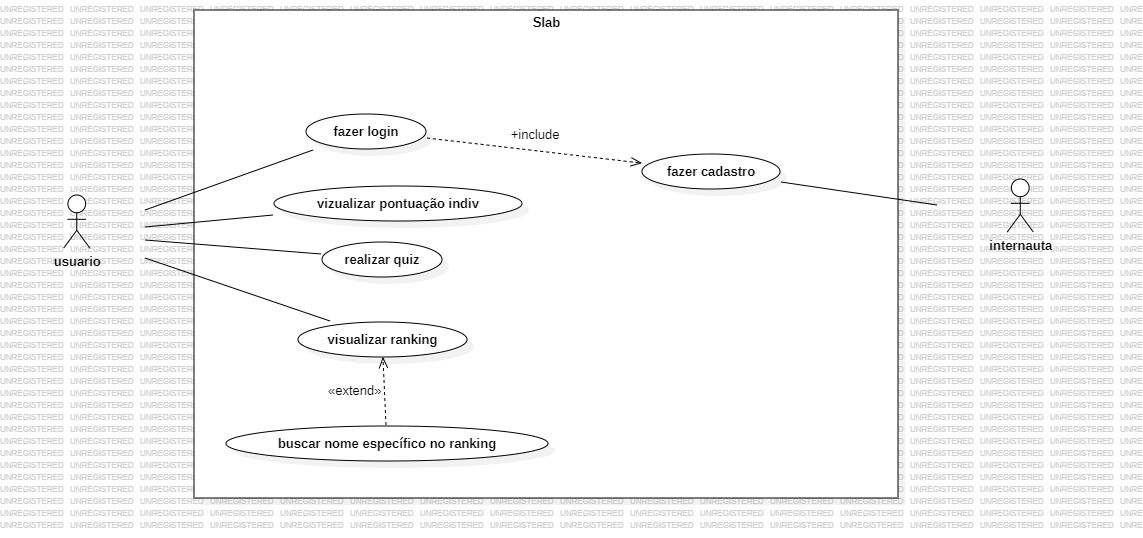
\includegraphics[width=1.1\textwidth]{imagens/UseCaseDiagram1}
\end{figure}

\begin{figure}
	\subsection{Diagrama de Classes}
  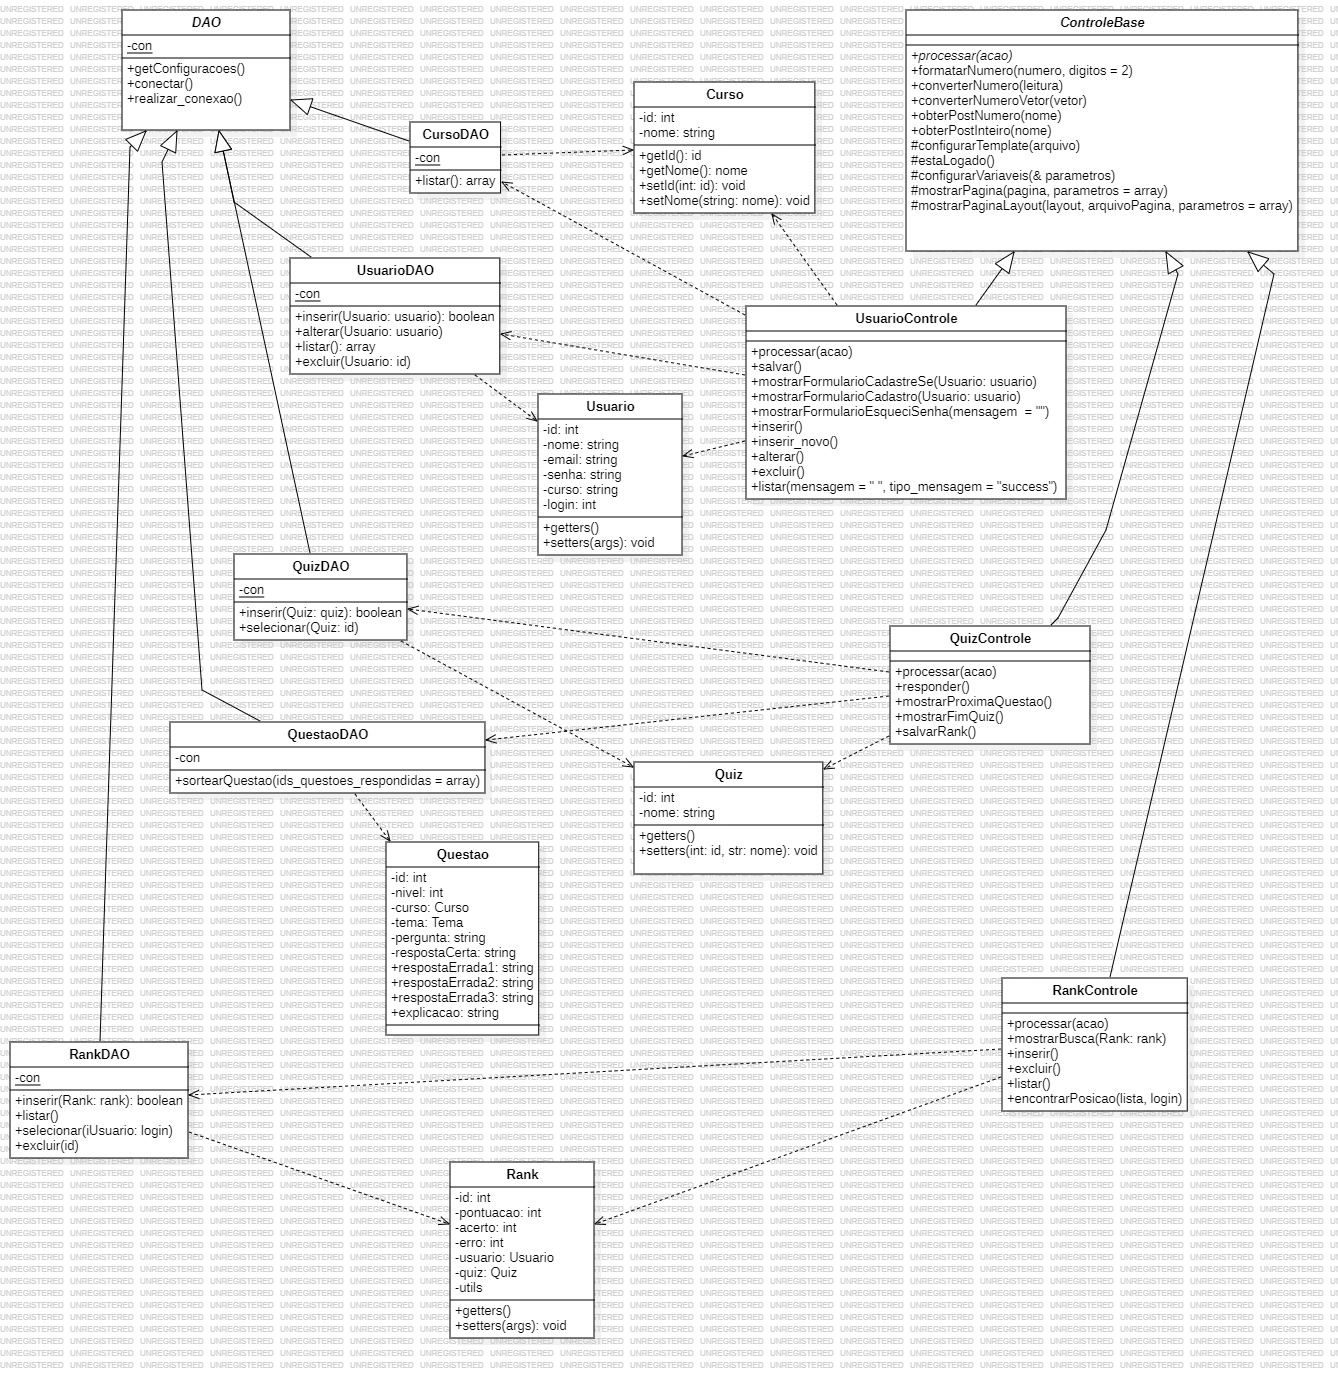
\includegraphics[width=1.1\textwidth,  keepaspectratio]{imagens/ClassDiagram1}
\end{figure}

\begin{figure}
	\subsection{Protótipos}
	\vspace{30pt}	
	
	\subsubsection{Cadastro do Usuário}
  	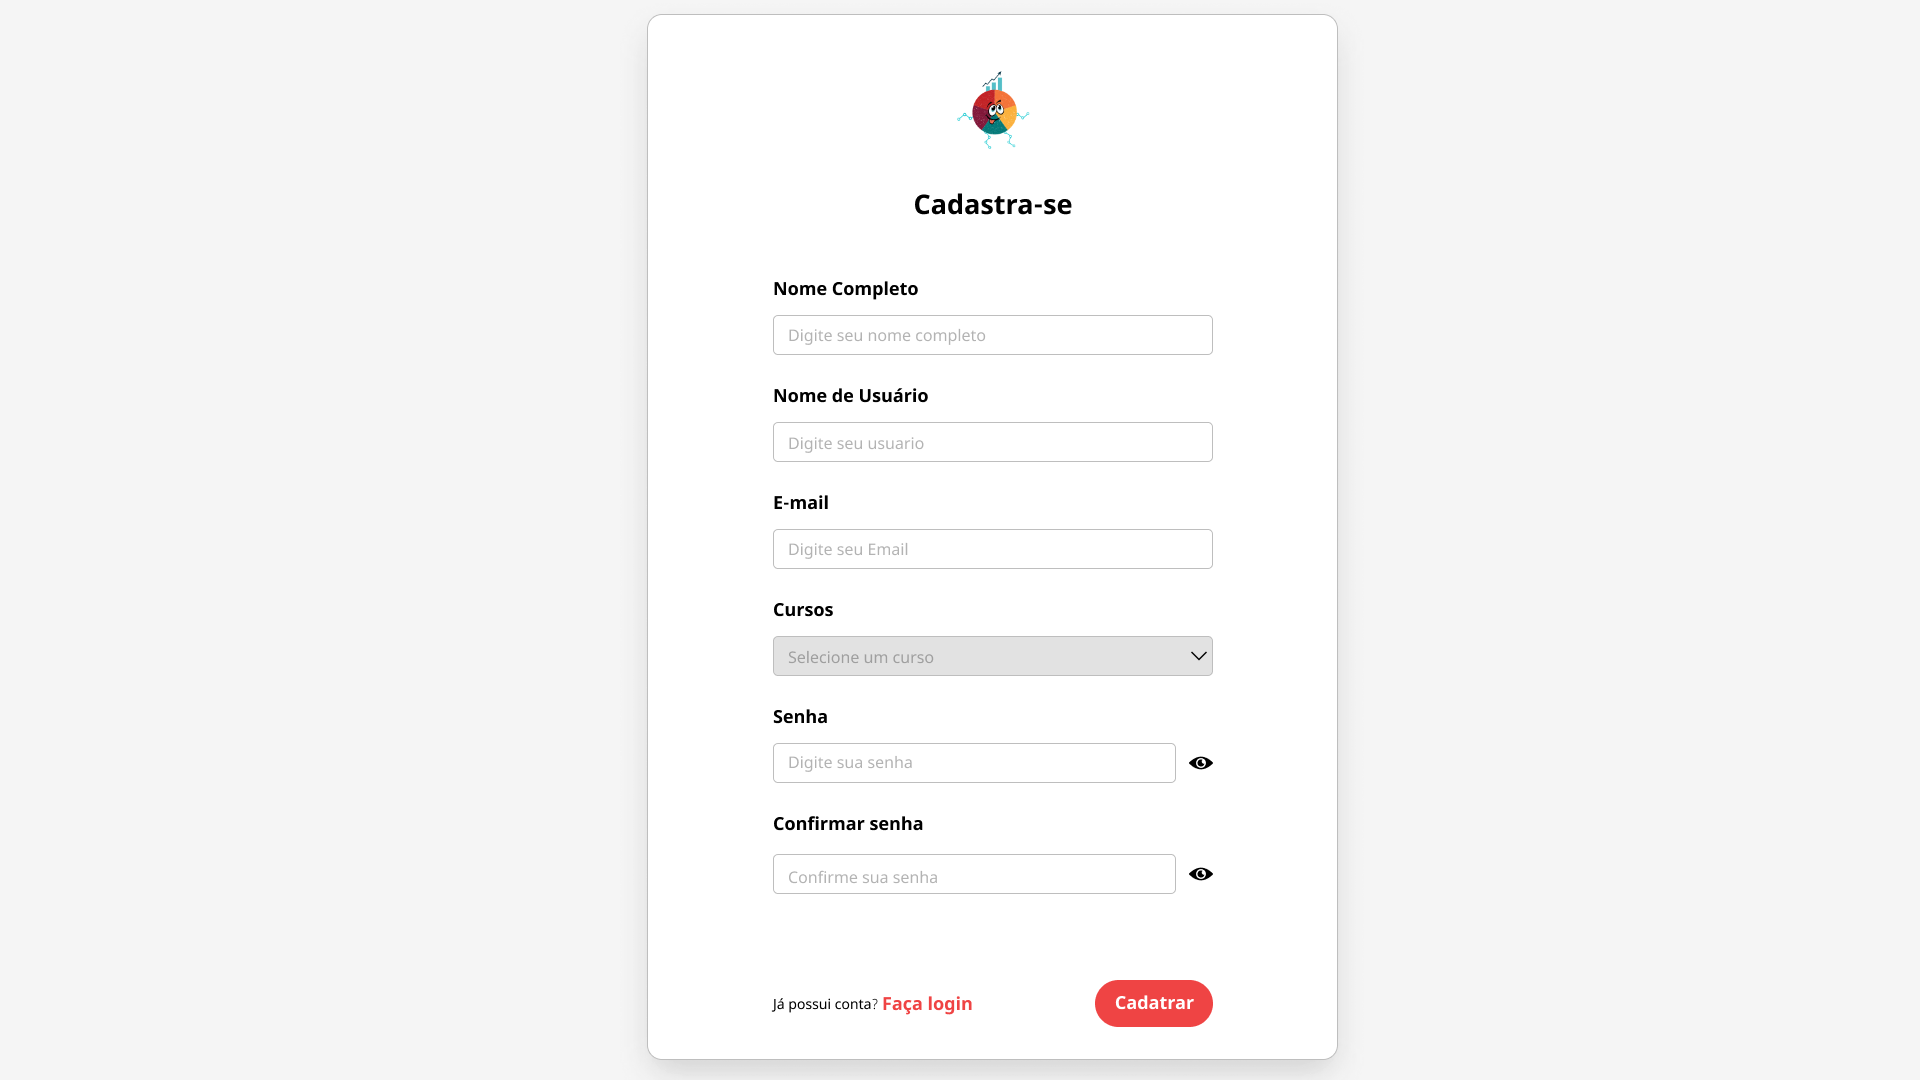
\includegraphics[width=\textwidth,  keepaspectratio]{imagens/Cadastro}
  	\vspace{30pt}
  	
  	\subsubsection{Login do Usuário}
  	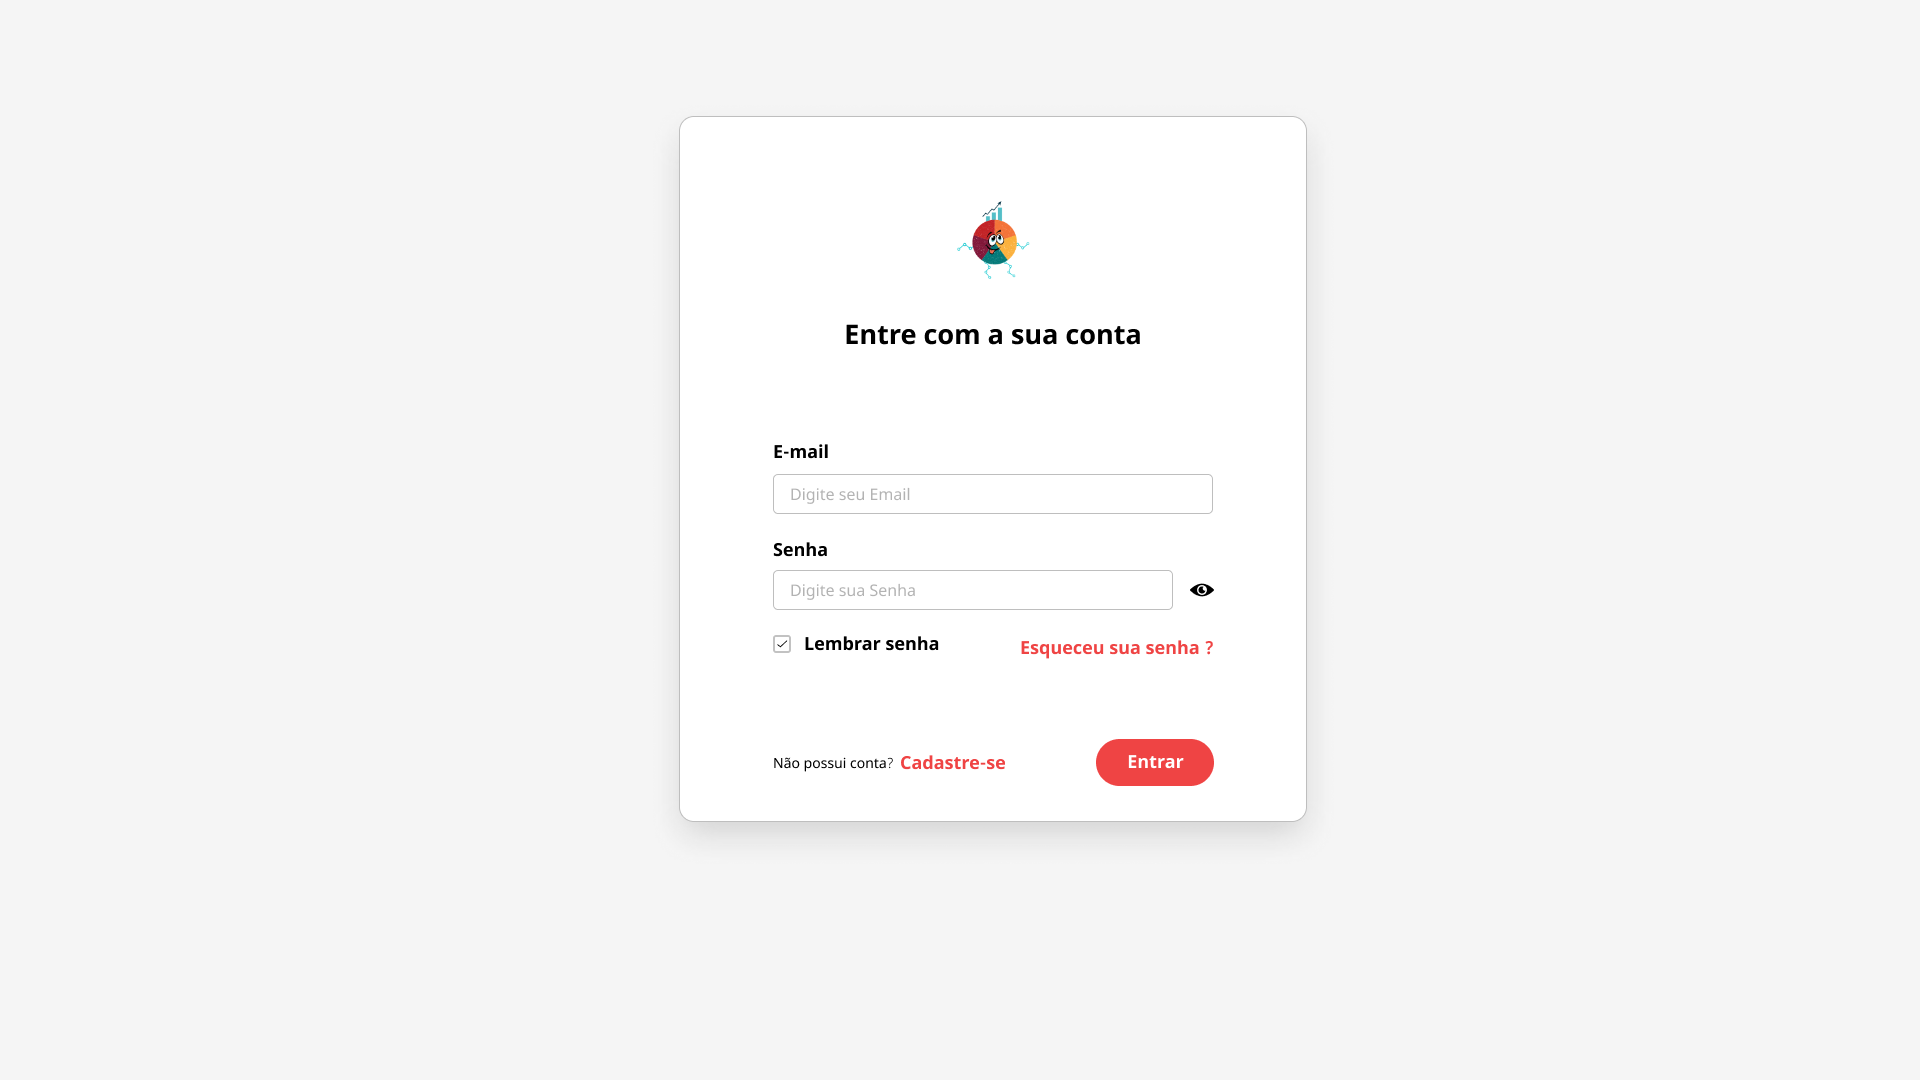
\includegraphics[width=\textwidth,  keepaspectratio]{imagens/Login}
	\vspace{30pt}
  	
\end{figure}

\begin{figure}
	\subsubsection{Ranking do Quiz}
  	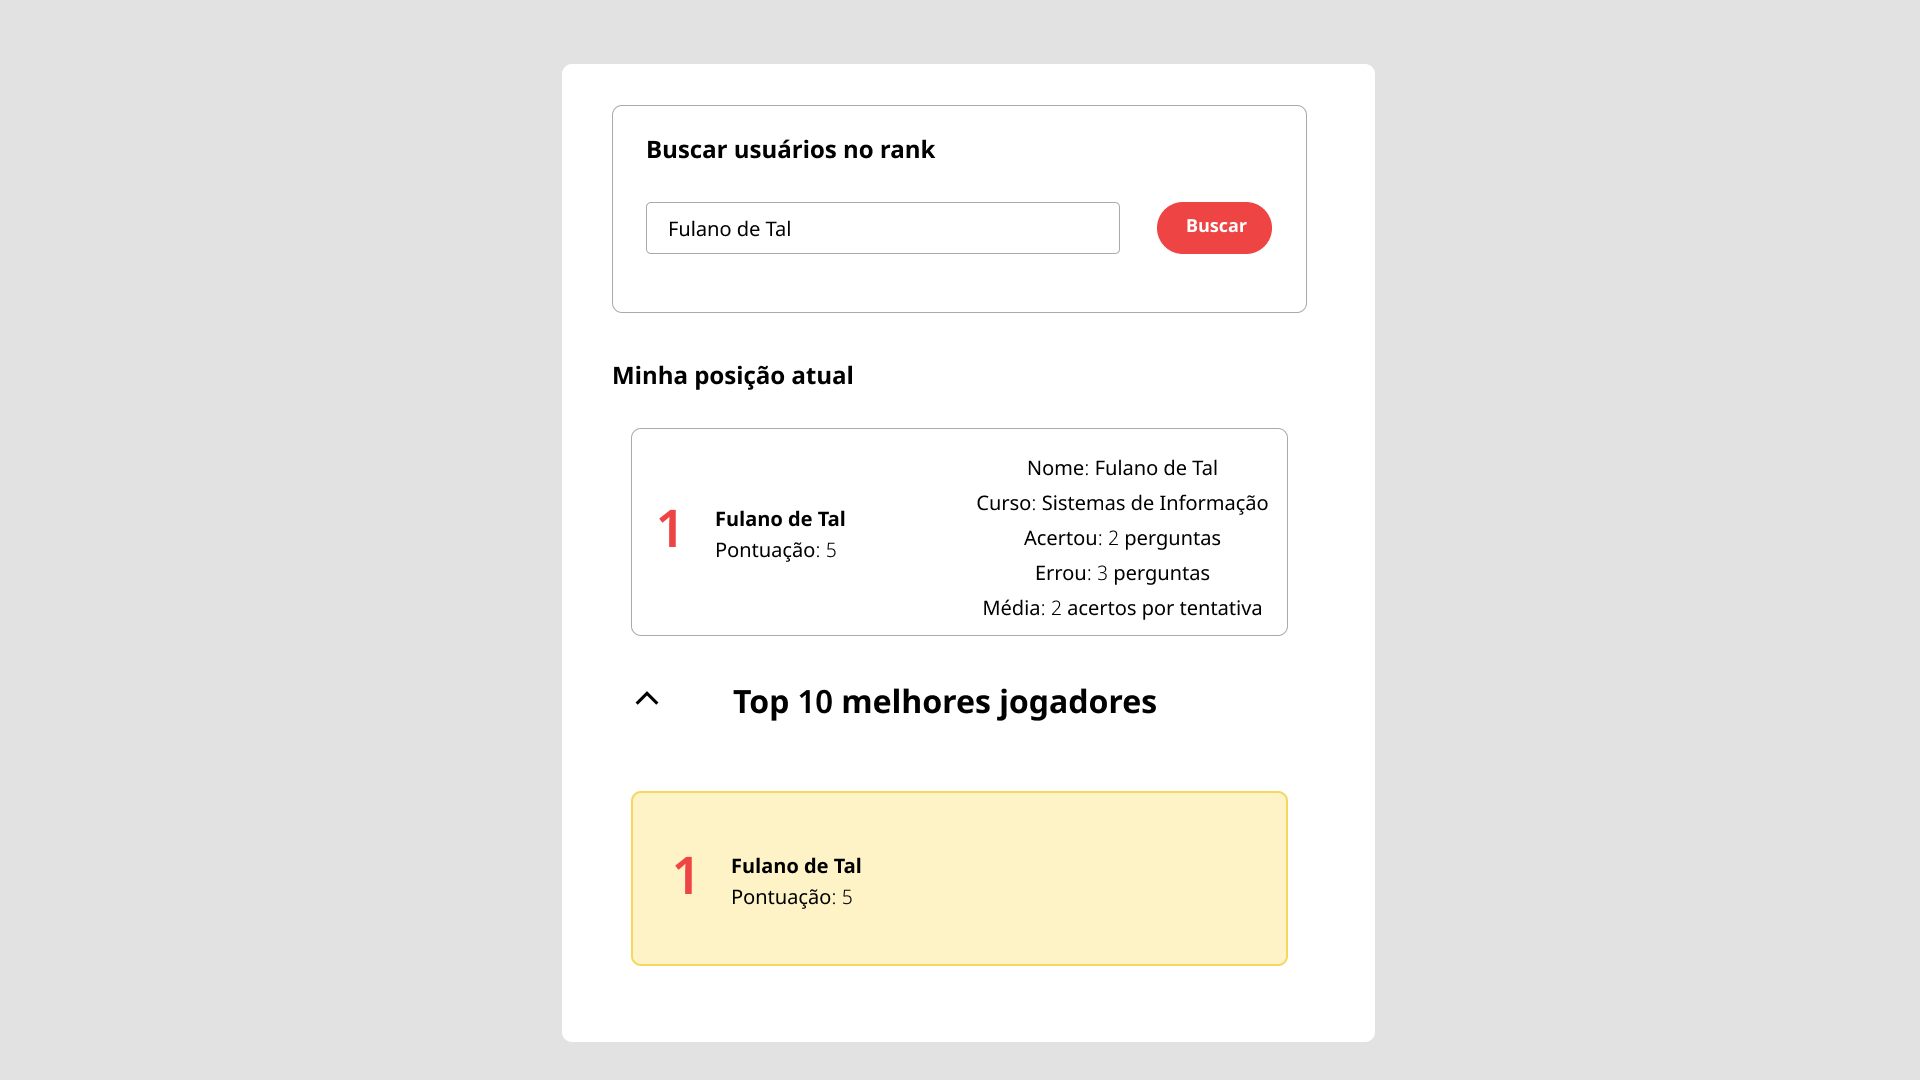
\includegraphics[width=\textwidth,  keepaspectratio]{imagens/Rank}
	\vspace{30pt}  	
  	
  	\subsubsection{Busca no Ranking}
  	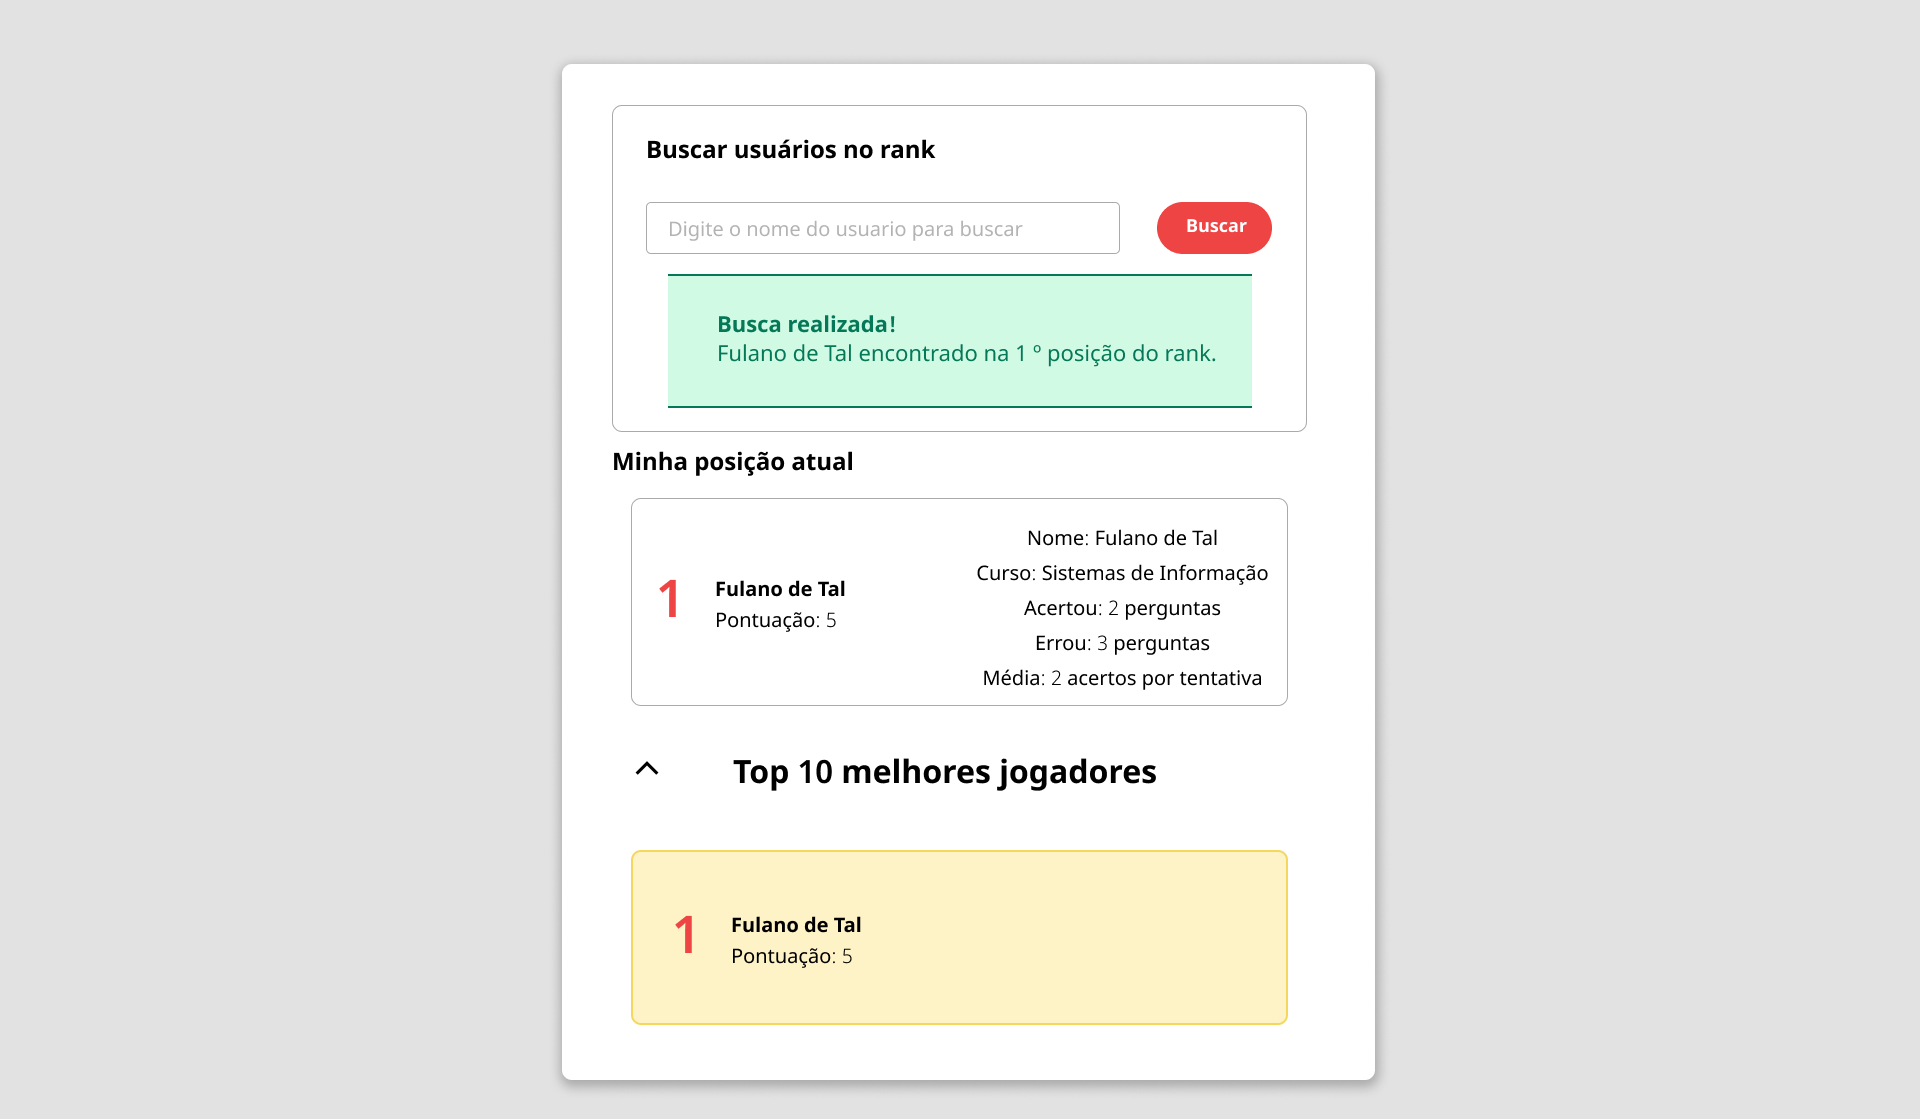
\includegraphics[width=\textwidth,  keepaspectratio]{imagens/Rank_busca}
	 	
\end{figure}

\end{document}
